\documentclass{article}
\usepackage{hyperref} 
\usepackage{graphicx}
\usepackage{float}
\usepackage{amsmath}
\usepackage{listings}
\usepackage{xcolor}
\usepackage{minted}
\usemintedstyle{colorful}

\title{Putnam Problem 1992 A6: Probability of Center Inside Tetrahedron}
\author{Dimitri Chrysafis}
\date{\today}

\begin{document}

\maketitle

\section{Introduction}
The Putnam problem 1992 A6 states: "Four points are chosen independently and at random on the surface of a sphere (using the uniform distribution). What is the probability that the center of the sphere lies inside the resulting tetrahedron?"

It can be proven by math that the answer is 1/8, or 0.125. In this text, we will present a computational approach to solve this problem. We will generate random points on a sphere, compute the resulting tetrahedron, visualize it, and determine the probability of the center lying inside the tetrahedron.

SOLUTION (NOT MINE) \href{https://dqlin.xyz/post/2018/09/01/putnam/}{https://dqlin.xyz/post/2018/09/01/putnam/}
\section{Examples}
Here are examples showing both cases: when the center of the sphere lies inside and outside the tetrahedron. Generated using plotly:

\begin{figure}[H]
    \centering
    \begin{minipage}[b]{0.45\textwidth}
        \centering
        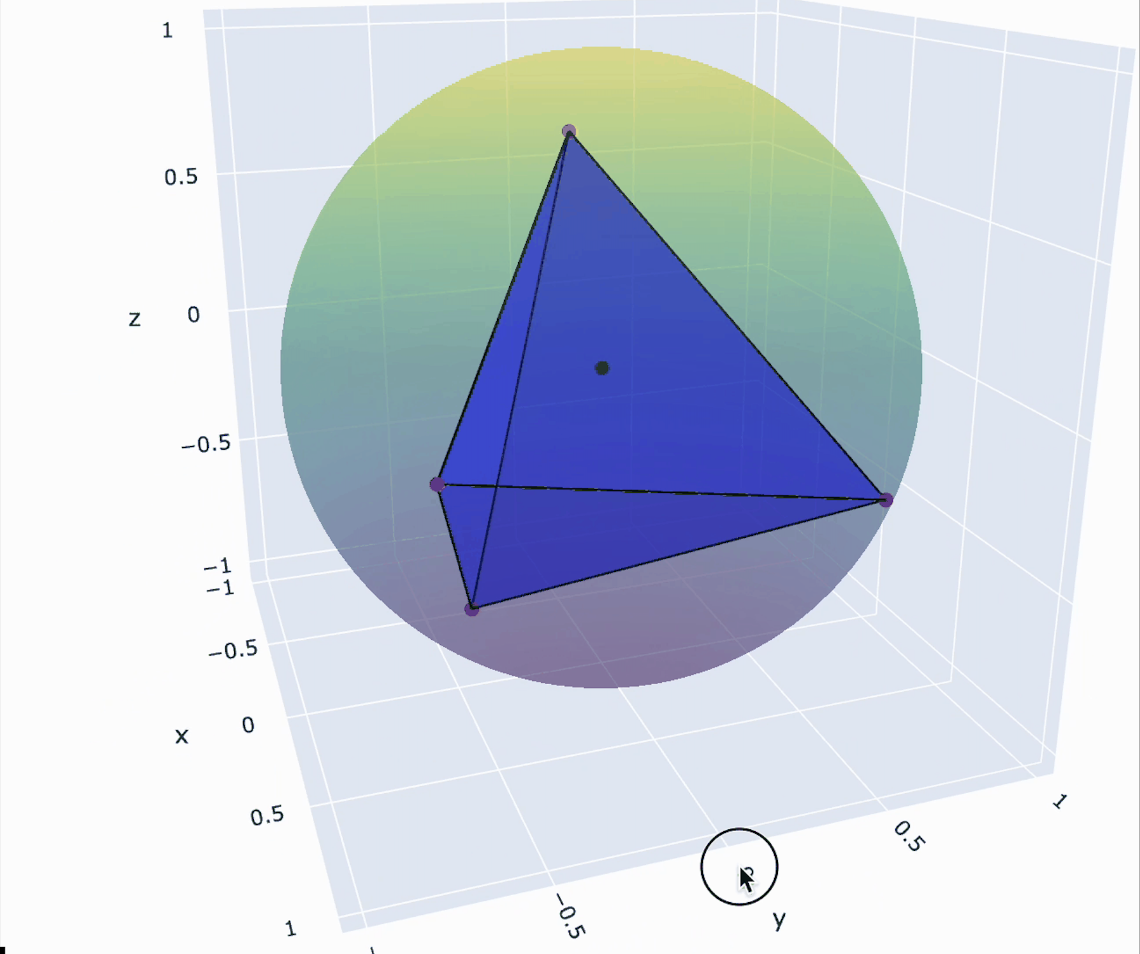
\includegraphics[width=\textwidth]{inside.png} 
        \caption{Center inside the tetrahedron.}
        \label{fig:center_inside}
    \end{minipage}
    \hfill
    \begin{minipage}[b]{0.45\textwidth}
        \centering
        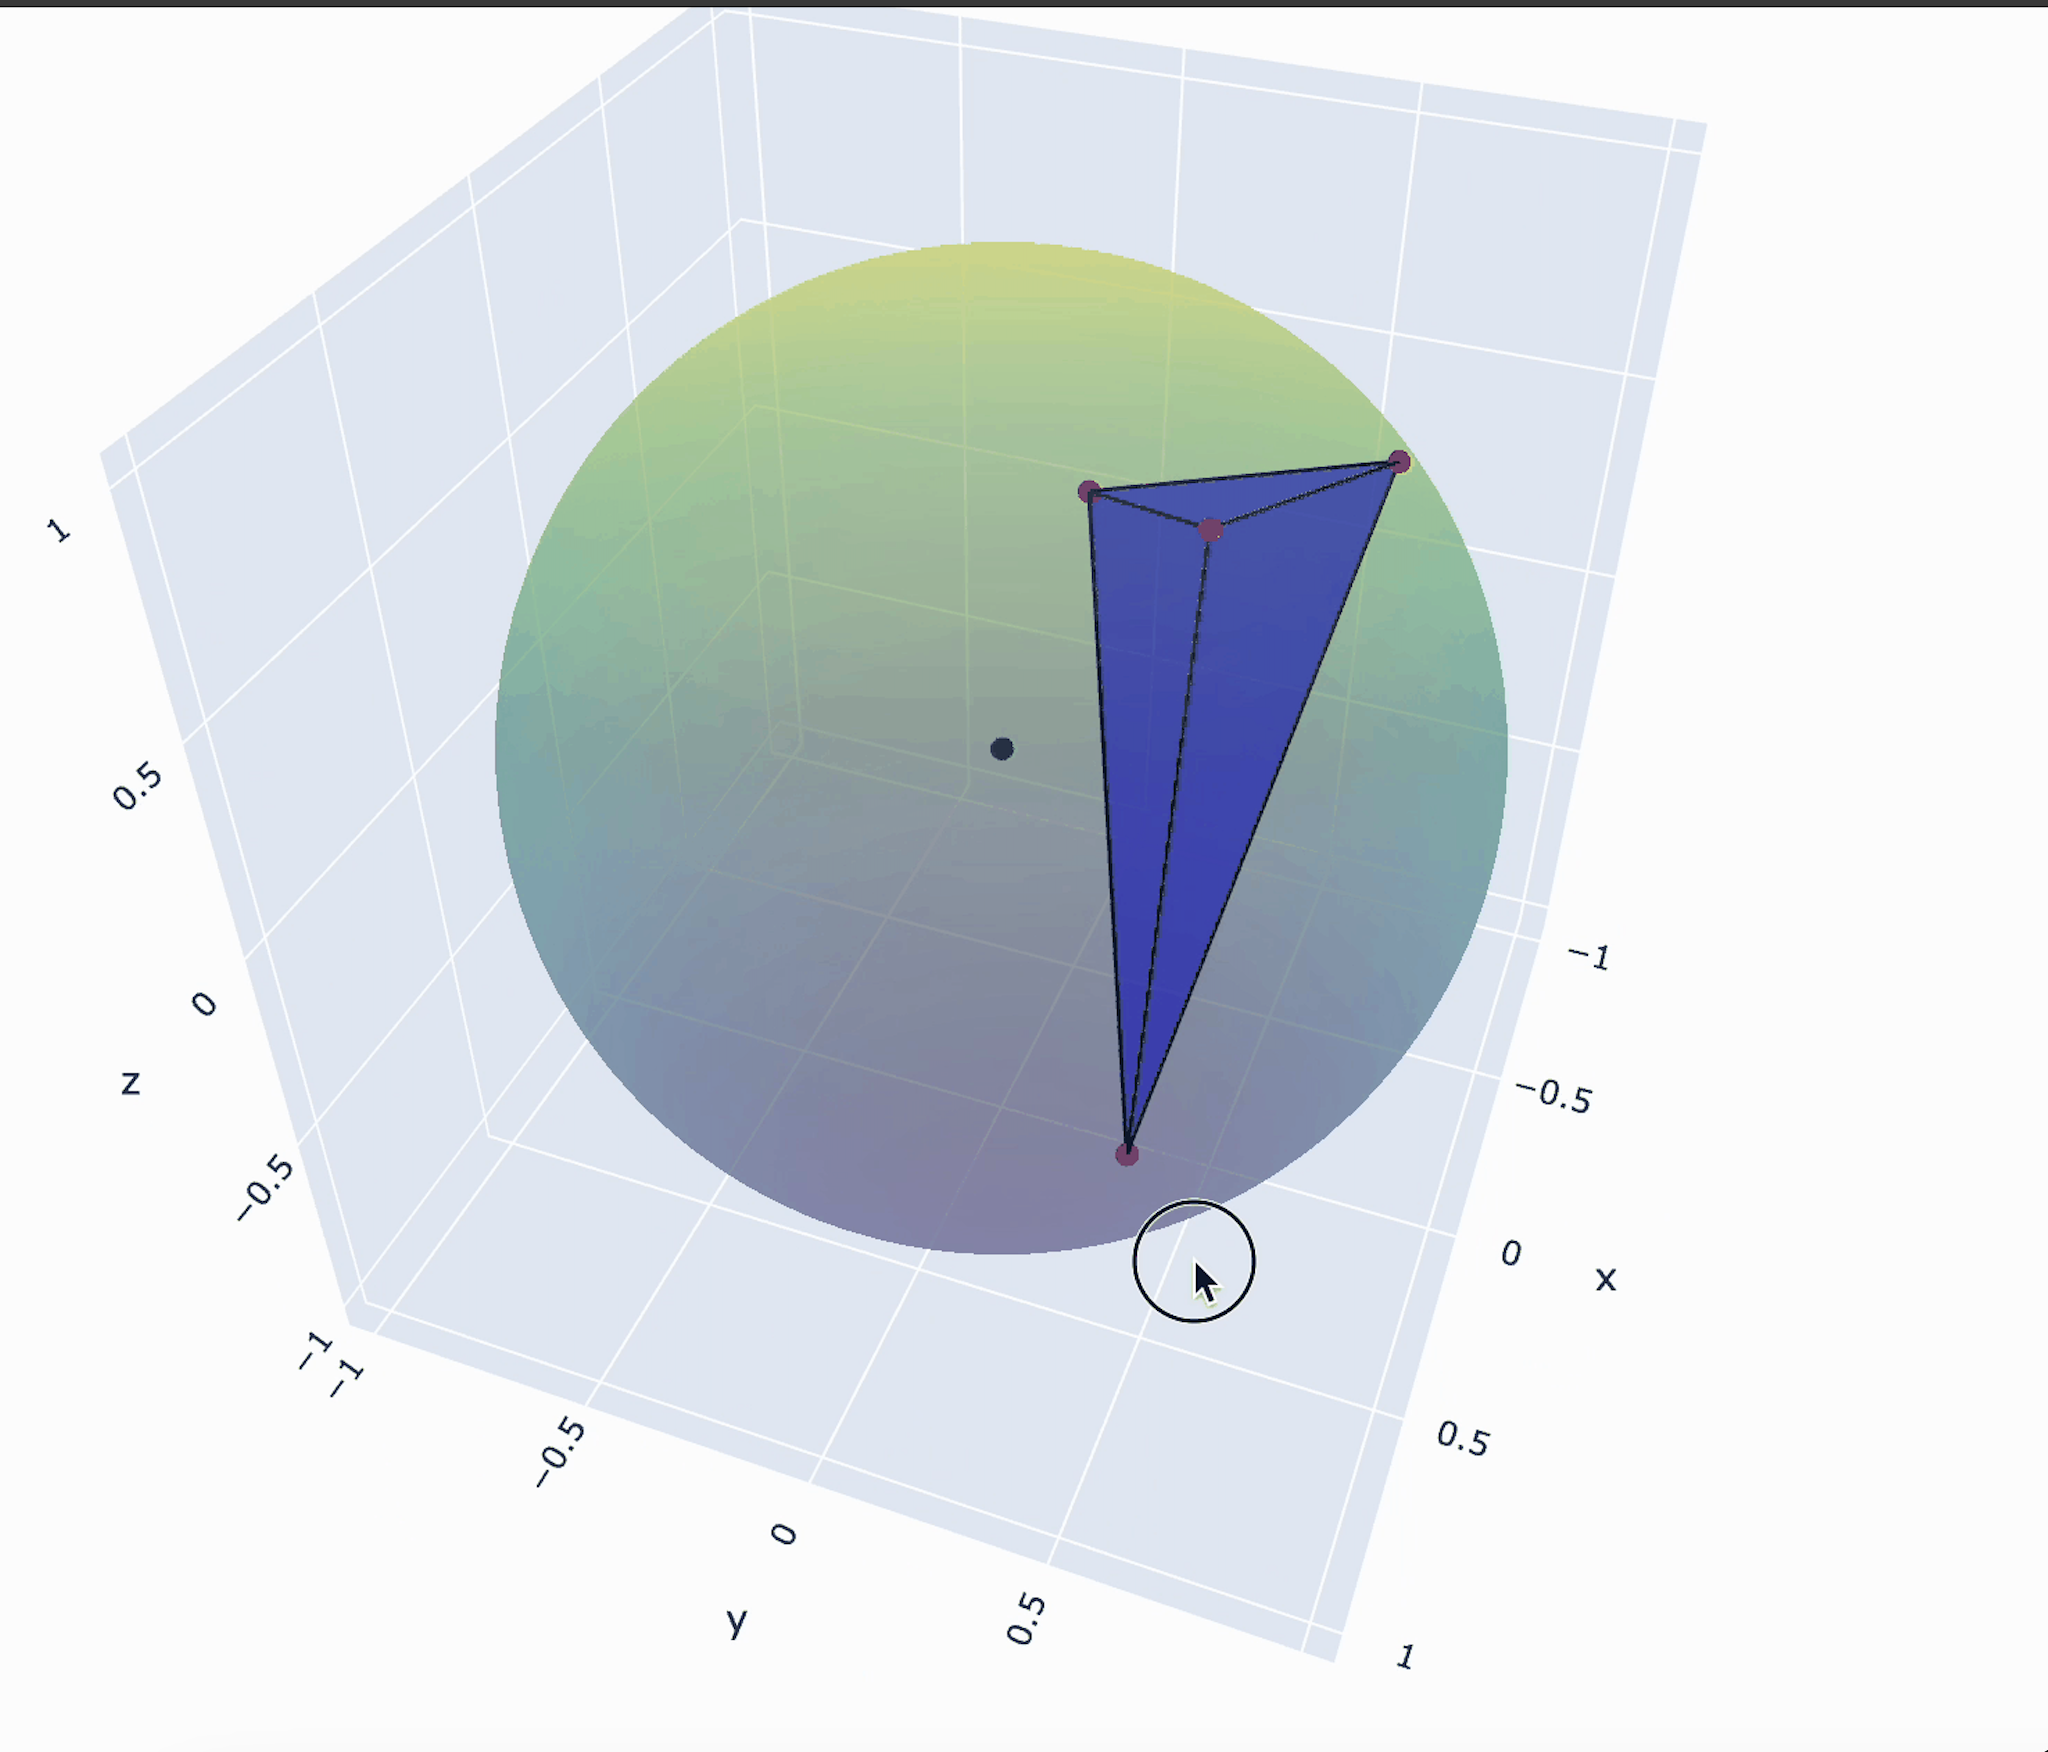
\includegraphics[width=\textwidth]{outside.png} 
        \caption{Center outside the tetrahedron.}
        \label{fig:center_outside}
    \end{minipage}
\end{figure}



\section{Methodology}
To solve the problem, we will follow these steps:

\begin{enumerate}
    \item Generate four random points on the surface of a sphere.
    \item Compute the convex hull of the points to form a tetrahedron rather than just four dots existing.
    \item Check if the center of the sphere lies inside the tetrahedron.
    \item Repeat the process for multiple simulations to calculate the probability.
\end{enumerate}

\section{Implementation Details}
We implemented the solution in Python using the following libraries:

\begin{itemize}
    \item \textbf{NumPy}: For numerical computations.
    \item \textbf{SciPy}: For computing the convex hull.
    \item \textbf{Matplotlib}: Running the 5000 image simulation to get the solution.
\end{itemize}

\section{Part 1: Simulation}

\subsection{Spherical Coordinates and Random Point Generation}

Spherical coordinates extend the concept of polar coordinates to represent points on a sphere in three-dimensional space.

In spherical coordinates:
\begin{itemize}
    \item \( r \) represents the distance from the origin.
    \item \( \theta \) is the angle from the positive x-axis in the xy-plane.
    \item \( \phi \) is the angle from the positive z-axis.
\end{itemize}

To generate random points uniformly distributed on the surface of a sphere:
\begin{enumerate}
  \item Generate a random azimuthal angle \( \phi \) uniformly between \( 0 \) and \( 2\pi \).
\begin{minted}[bgcolor=lightgray]{python}
phi = np.random.uniform(0, 2*np.pi, num_points)
\end{minted}

    
 \item Generate a random polar angle \( \theta \) by sampling \( \cos(\theta) \) uniformly between \( -1 \) and \( 1 \), then calculate \( \theta = \arccos(\cos(\theta)) \).
\begin{minted}[bgcolor=lightgray]{python}
cos_theta = np.random.uniform(-1, 1, num_points)
theta = np.arccos(cos_theta)
\end{minted}

    
    \item Convert spherical coordinates to Cartesian coordinates \( (x, y, z) \).
    \begin{minted}[bgcolor=lightgray]{python}
    points /= np.linalg.norm(points, axis=1)[:, np.newaxis]
    \end{minted}

\end{enumerate}

This method provides us with random points uniformly distributed on the surface of the sphere.



\subsection{Checking If Center Is Inside}

To determine if the center of the sphere lies inside the tetrahedron, we utilize the convex hull of the generated points. Here's how the process works:

First, let's examine the \texttt{isInCenter} function:

\begin{minted}[bgcolor=lightgray]{python}
def isInCenter(points):
    hull = ConvexHull(points)
    center = np.array([0, 0, 0])
    equations = hull.equations
    signs = np.sign(np.dot(equations[:, :-1], center) + equations[:, -1])
    return np.all(signs <= 0) or np.all(signs >= 0)
\end{minted}

Here's how it works:
\begin{enumerate}
    \item We compute the convex hull of the points using \texttt{scipy.spatial.ConvexHull}.
    \item Next, we obtain the equations of the planes defining the convex hull.
    \item Then, we calculate the signed distances from the center of the sphere to these planes.
    \item If all signs are less than or equal to zero, or all signs are greater than or equal to zero, it indicates that the center lies inside the convex hull (tetrahedron).
\end{enumerate}

This method works because if the center lies inside the tetrahedron, it will have the same sign for all distances to the planes formed by the tetrahedron's faces. Otherwise, if it lies outside, the signs will differ.

\subsection{Generating the Images and Multithreading}

This function generates a 3D plot of the tetrahedron and the sphere with annotations indicating the result of each simulation iteration. It includes:
\begin{itemize}
    \item Wireframe of the sphere.
    \item Convex hull of the points forming the tetrahedron.
    \item Scatter plot of the random points.
    \item Annotation for the center of the sphere.
    \item Annotation showing the current index, probability, and whether the center is inside or outside the tetrahedron.
    \item Table showing the coordinates of each point.
    \item Finally, it saves the plot as an image file for later reference and conversion into a video.
\end{itemize}

We use the multiprocessing module in Python to divide the simulation workload among multiple CPU cores. Here's the code snippet:

\begin{minted}[bgcolor=lightgray]{python}
import multiprocessing

def simulate_single(max_size_bytes):
    # Simulation code
    pass

def compileSize(max_size_bytes=1000000000):
    num_cores = multiprocessing.cpu_count()
    pool = multiprocessing.Pool(processes=num_cores)
    results = pool.map(simulate_single, [max_size_bytes] * num_cores)
    pool.close()
    pool.join()

    probability = sum(results) / len(results)

    print(f'Final Result {probability:.6f}')
\end{minted}

The \texttt{compileSize} function creates a pool of processes, maps the \texttt{simulate\_single} function to each process, and runs them concurrently. This maximizes CPU utilization and speeds up the simulation.

\section{Conclusion/Data}
When running this code in python, I could only get to case 33800000.png which will be shown below. The c++ did not have to render images and only captured instances every million or so, as can be seen in the output. It is unknown why the probabilities were so different.

\begin{figure}[H]
    \centering
    \begin{minipage}[b]{0.45\textwidth}
        \centering
        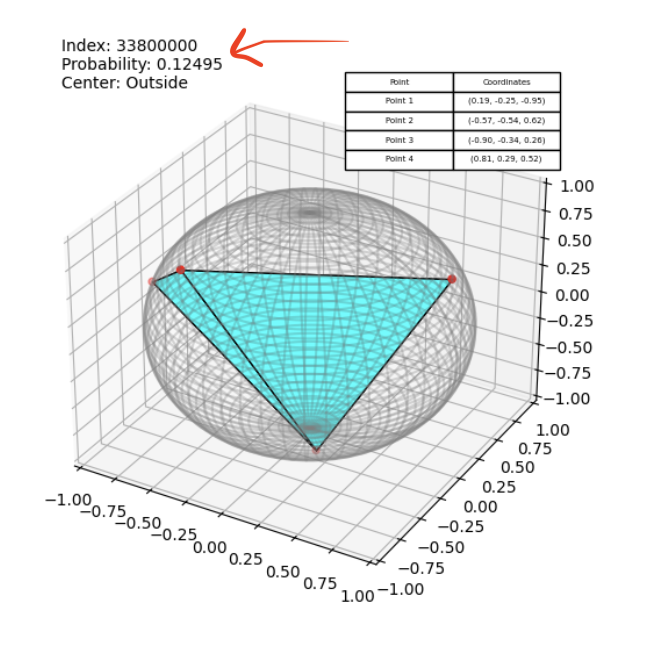
\includegraphics[width=\textwidth]{tetrahedron_33800000.png} 
        \caption{Python Version (Higher accuracy)}
        \label{fig:center_inside}
    \end{minipage}
    \hfill
    \begin{minipage}[b]{0.45\textwidth}
        \centering
        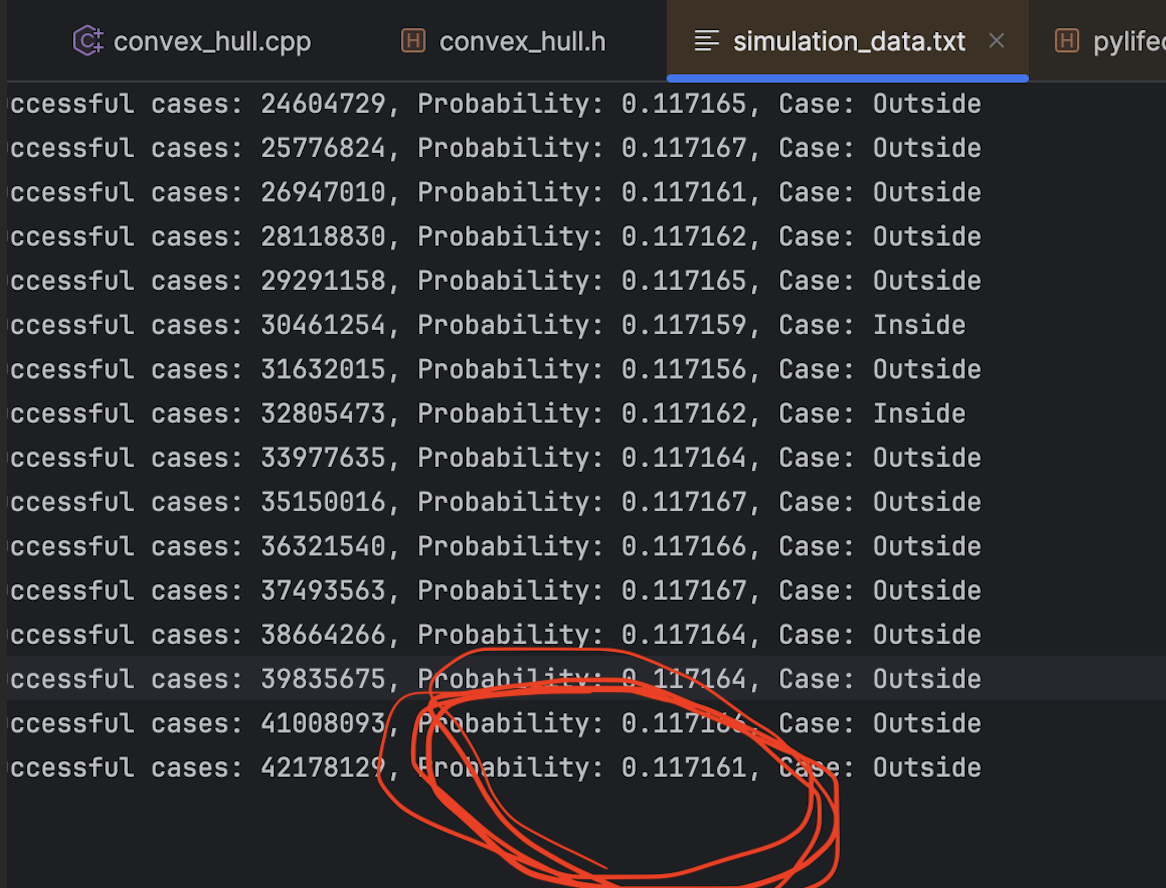
\includegraphics[width=\textwidth]{c++version.png} 
        \caption{C++ Version (Much faster yet off by 0.008 ish}
        \label{fig:center_outside}
    \end{minipage}
\end{figure}


\section{Extras}

In addition to the main simulation, I explored two additional visualization methods: one using Plotly for interactive 3D visualization and another using Pygame to render images into a video.

\subsection{Plotly 3D Interactive Playground}
For interactive visualization, I utilized Plotly, a powerful Python library. Here's how I implemented it:

\begin{itemize}
    \item Generated random points on the surface of a sphere using polar coordinates.
    \item Rendered the sphere and the convex hull formed by these points using Plotly.
    \item Created an interactive 3D playground where the scene could be rotated, zoomed, and explored dynamically. (on page below) (compile code to actually play with it)
\end{itemize}
\begin{figure}[H]
    \centering
    \begin{minipage}[b]{0.9\textwidth}
        \centering
        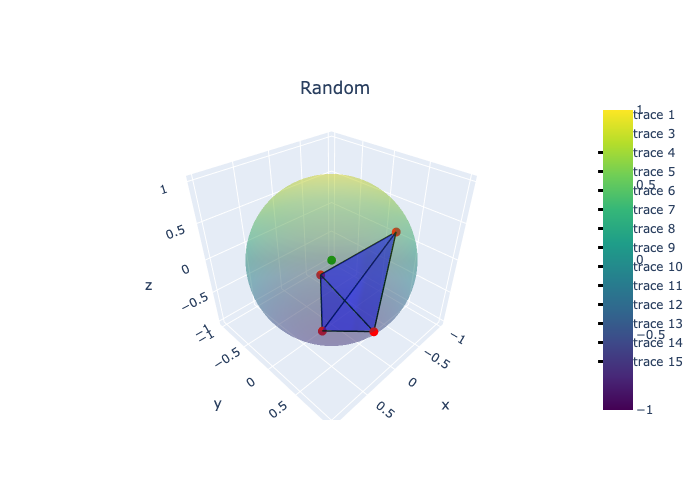
\includegraphics[width=\textwidth]{plotly.png} 
        \caption{Python Version (Higher accuracy)}
        \label{fig:center_inside}
    \end{minipage}
\end{figure}


This was mostly for me to experiment with the sphere stuff. 

\subsection{Pygame Image Renderer}
To create a video of the simulation, I used Pygame, a popular library for game development. Here's what I did:

\begin{itemize}
    \item generated random points on the sphere's surface and calculated the convex hull.
    \item saved each visualization as an image file in a folder.
    \item had Pygame to render these images sequentially, creating a video of the evolving scene.
    \item https://github.com/DimitriChrysafis/Putnam1992A6/blob/main/input.gif
    \item THE GIF IT GENERATES CAN BE FOUND ABOVE 
\end{itemize}

the approach gave the for the generation of a video that visualized the simulation process step by step


\section{Code}
The code for this project is available on GitHub: \texttt{https://github.com/DimitriChrysafis/Putnam1992A6/tree/main}

\section{Final Simulation Youtube}
\href{https://www.youtube.com/watch?v=JD38GMMxUhc}{Click here to watch the video}

\end{document}